% Drawing 67/05-6 -- folder 67, batch 05, archive page 99 (PDF page 100).
% Transcription: dans la marge gauche, sous le mot « Démonstration » : l'hexagone, sommets notés $v - u$ et $v$ en haut, $-u$ à gauche, « $e_{0} = u_{+}$ » à droite (au bout d'une flèche épaisse issue du centre, sous laquelle est écrit $e_{0}$), $-v$ et « $\sigma v = u - v$ » en bas ; au-dessus, le sommet du triangle extérieur, noté « $2v - u = u_{-}$ » après un mot biffé ; des traits et des flèches vont du centre aux sommets, un axe vertical en tirets descend du sommet du triangle au centre.
% Kind: hexagon with named vertices, arrows from the centre, outer apex u_-. Method 2 (schematic redraw from the facsimile). Status: partial.
% Notes: As on the page, with every stroke between the same computed vertices: the outer triangle on the top side (its two sides from v-u and v to the apex, labelled « 2v-u = u_- »); the top side, dashed; the sides v-u to -u, v to e_0 = u_+, e_0 to u-v, -u to -v and the bottom side; the heavy arrow from the centre to e_0 = u_+, with e_0 written under it; arrows from the centre to -v and to u-v; plain strokes from the centre to v-u, to v and to -u; the dashed vertical axis from the apex to the centre. Labels where he wrote them. Left out: the struck word before « 2v-u », a struck sign inside the triangle, a short dashed vertical under v, and the word « Démonstration » above. Still differs: which of the strokes from the centre carry an arrowhead is a reading (heads are clear on e_0, -v and u-v; the stroke from -u towards v-u also seems to carry a head, not drawn); the label at the upper right vertex is overwritten and is given after the transcription as v. Redrawn 2026-11-12 (issue 128): to check again.
% Coordinates: 1 unit = 1 mm = 1/100 of the crop width (bbox in page fractions: [0.1, 0.58, 0.32, 0.75]).
% Redrawn by Claude (claude-fable-5-2), issue #128, 2026-11-12; not checked by a human; not compiled (no TeX in the session).
% Rights: reproduces part of the work -- behind RENDER_TRANSCRIPTS, never published by itself.
\documentclass[tikz,border=3pt]{standalone}
\usepackage{amsmath,amssymb}
\usetikzlibrary{patterns,arrows.meta}
\tikzset{pencil/.style={black!45}, struck/.style={black!35}, mpt/.style={circle,draw,inner sep=1.3pt}, pt/.style={circle,fill,inner sep=0.9pt}, opt/.style={circle,draw,fill=white,inner sep=1.1pt}}
\begin{document}
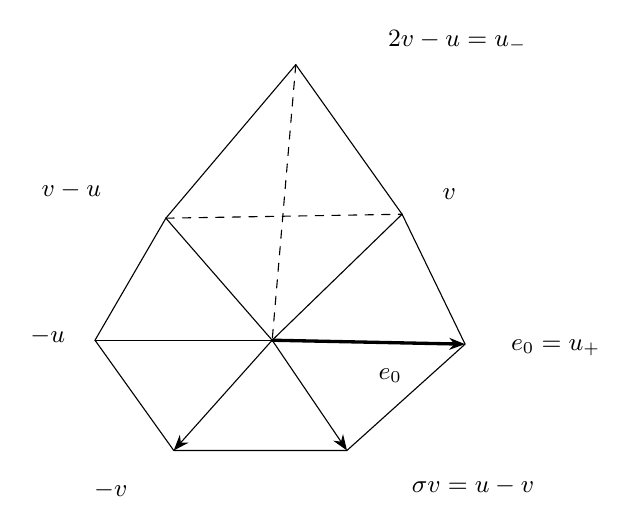
\begin{tikzpicture}[x=1mm,y=1mm,line cap=round,line join=round,font=\scriptsize]
\draw (42,-55) -- (58.5,-35.5) -- (72,-54.5);
\draw[dashed] (42,-55) -- (72,-54.5);
\draw (42,-55) -- (33,-70.5) -- (43,-84.5) -- (65,-84.5) -- (80,-71) -- (72,-54.5);
\draw[very thick,-{Stealth[length=2mm]}] (55.5,-70.5) -- (80,-71);
\draw[-{Stealth[length=2mm]}] (55.5,-70.5) -- (43,-84.5);
\draw[-{Stealth[length=2mm]}] (55.5,-70.5) -- (65,-84.5);
\draw (55.5,-70.5) -- (42,-55);
\draw (55.5,-70.5) -- (72,-54.5);
\draw (55.5,-70.5) -- (33,-70.5);
\draw[dashed] (58.5,-35.5) -- (55.5,-70.5);
\node[inner sep=1pt] at (79,-32.5) {\small $2v-u=u_{-}$};
\node[inner sep=1pt] at (30,-51.5) {\small $v-u$};
\node[inner sep=1pt] at (78,-52) {\small $v$};
\node[inner sep=1pt] at (27,-70) {\small $-u$};
\node[inner sep=1pt] at (70.5,-75) {\small $e_{0}$};
\node[inner sep=1pt] at (91.5,-71.5) {\small $e_{0}=u_{+}$};
\node[inner sep=1pt] at (35,-89.5) {\small $-v$};
\node[inner sep=1pt] at (81,-89) {\small $\sigma v=u-v$};
\end{tikzpicture}
\end{document}
